

\chapter{Repairing Strategy : Bounded Forward and Backward Analysis}
\label{chapter:boundedAnalysis}


\section{Example Scenario}
\label{exampleScenario}

We have performed dataflow analysis by extending Soot main class. The objectives
of the dataflow analysis are the following:

\begin{itemize}
  \item For a target statement analyze used and defined variables.
  
  \item Extracts other statements which are both above and bellow the target
  statement in the control flow graph on which the used and defined variables
  are dependent on.
  
\end{itemize}

In the code snippet~\ref{dataflow}, we gave an example code based on java
\emph{String} API to demonstrate the analysis.

\onehalfspacing
\lstset{language=Java, caption=Dataflow analysis,
label=dataflow}
\begin{lstlisting}
void bar()
{
  foo("fname:lname");
}

String foo(String s)
{
  int a = s.indexof(":");
  int b = s.indexOf("&");
  int c = s.indexOf("#");
  int d = 0;
  if(c>0)
  {
    d = 1;
  }
  return s.substring(a,b);
}

\end{lstlisting}

Let us assume that our target is \texttt{s.substring(a,b)} which in this case
may throw an array index out of bound exception. In this target statement,
\texttt{a} and \texttt{b} are used variable which are dependent on another
String API method i.e \texttt{indexOf()} which calculates index of starting of a
sub-string or single character in the main string. In case the sub-string or the
character does not exist in the main string, \texttt{indexOf()} method returns
$-1$ which causes throwing a runtime exception in the \texttt{substring()}
method call.
\newline
By using dataflow analysis we try to understand how these different variables
are corelated and based on that how we can effectively apply patching technique
so the patching code will have very less footprint in the instrumented bytecode.

\section{Flow Functions}
\label{flowFunctions}

\begin{figure}[b]
\centering
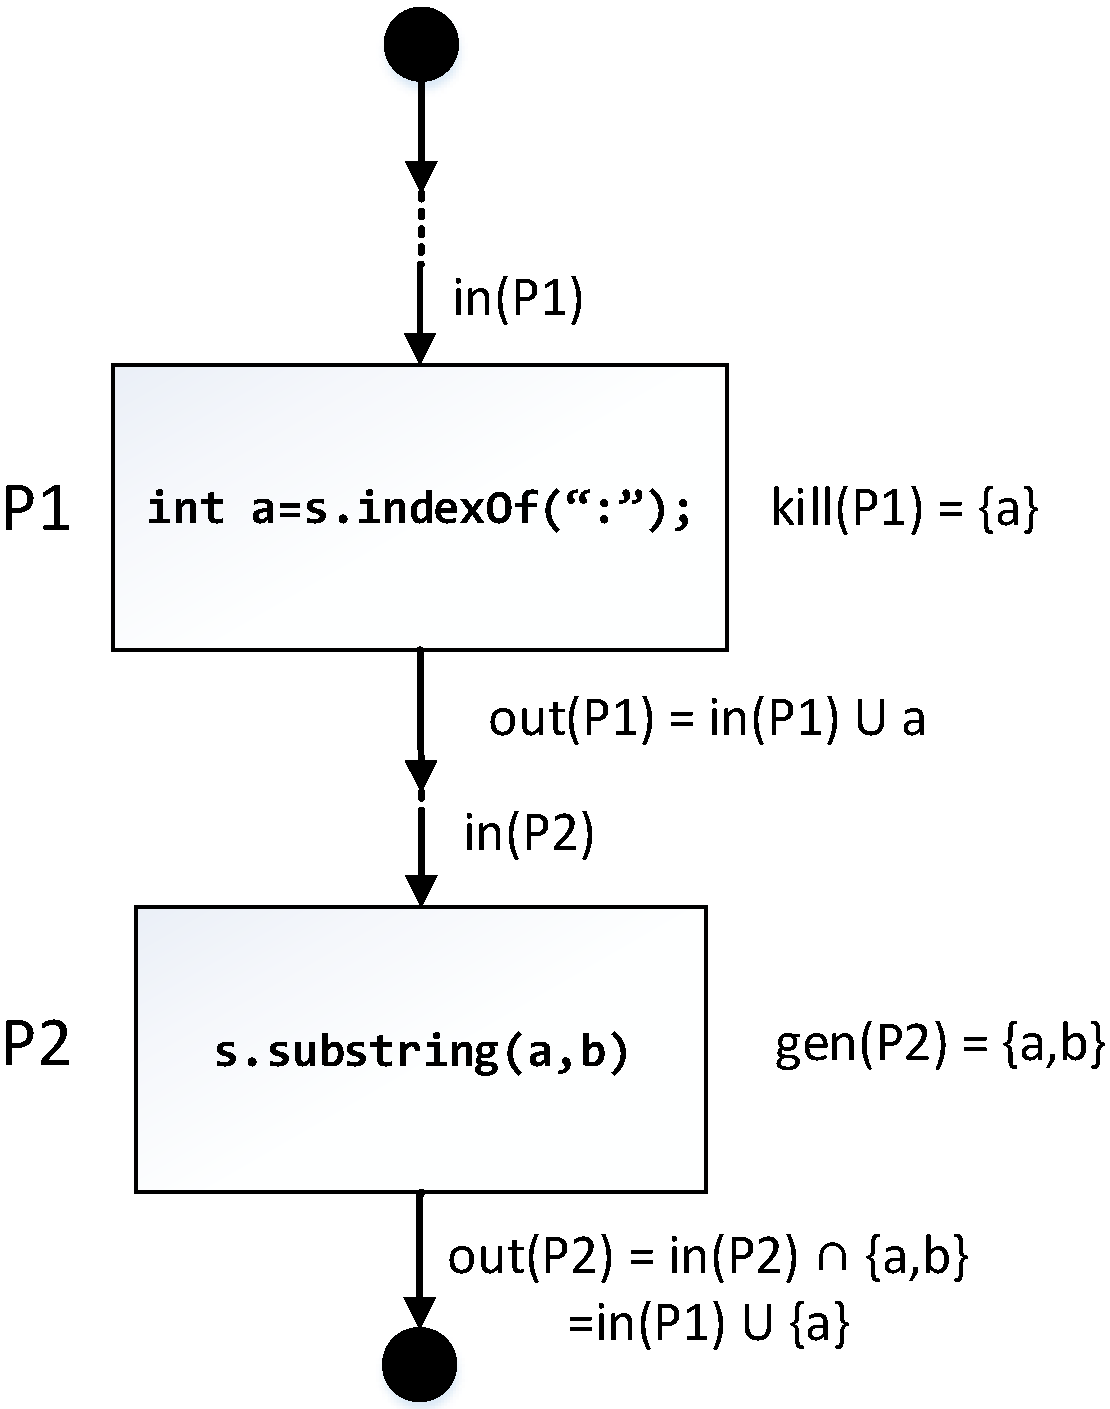
\includegraphics[width=1.8in]{images/dataflow.png}
\caption{Dataflow diagram with in, out set}
\label{fig:dataflow}
\end{figure}


Let us define $p$ as a program point/ node in the control flow graph. $in(P)$
and $out(P)$ respectively denotes in set and out set to and from the node $P$.
We define set $IG$ as the set of methods like \texttt{indexOf()},
\texttt{codePointAt()}, \texttt{CodePointBefore()} etc. which returns an integer
which can be used as input to other String methods. We also define set $IU$
which contains the methods which may use the integers produced by the methods in
$IG$ Then, 
$$out(P) = in(P) \cup kill(P)$$ where statement in P is a invoke statement and
method $m \in IG$ and
$$out(P) = in(P) \cap gen(P)$$ where statement in P is a invoke statement and
method $m \in IU$. Initial entry set = ${\phi}$.

In the figure~\ref{fig:dataflow}, we gave an example of a sample CFG whin in set
and out set.
